
A legislação fiscal brasileira é notoriamente conhecida por ser complexa. Nas duas últimas décadas, representantes das três esferas do governo brasileiro, municipal, estadual, e federal, se reuniram para tentar mudar essa realidade promovendo uma atuação mais integrada e modernizando o sistema. O mercado brasileiro também respondeu a essas mudanças criando oportunidades que visam facilitar o cumprimento das obrigações fiscais de empresas de todo país.

\section{Legislação Brasileira}
\label{section:documentos-fiscais:legislacao}

O Sistema Tributário Nacional foi instituído pela lei nº 5172 de 1966 \cite{lei:5172:codigo-tributario}, há mais de cinco décadas. Desde então passou por diversas reformas visando aumentar sua eficiência, modernizando-o. O artigo 37 da Constituição Federal, alterado pela Emenda Constitucional nº 42 de 19 de dezembro de 2003 \cite{constituicao:emenda42_2003}, em seu vigésimo segundo inciso prevê:

\begin{citacao}
Art. 37. A administração pública direta e indireta de qualquer dos Poderes da União, dos Estados, do Distrito Federal e dos Municípios obedecerá aos princípios de legalidade, impessoalidade, moralidade, publicidade e eficiência e, também, ao seguinte:

...

XXII - as administrações tributárias da União, dos Estados, do Distrito Federal e dos Municípios, atividades essenciais ao funcionamento do Estado, exercidas por servidores de carreiras específicas, terão recursos prioritários para a realização de suas atividades e atuarão de forma integrada, inclusive com o compartilhamento de cadastros e de informações fiscais, na forma da lei ou convênio \cite{constituicao:1988}.
\end{citacao}

O compartilhamento de cadastros e de informações previsto neste artigo permitiu então que as esferas do governo brasileiro tomassem atitudes no sentido de centralizar sistemas tributários, criando protocolos e sistemas para tal.

Desde então, diversos secretários da Fazenda Federal, das Fazendas Estaduais e do Distrito Federal, e de Fazendas Municipais se reúnem anualmente no \sigla{ENAT}{Encontro Nacional de Administradores Tributários} para discutir como modernizar e tornar mais efetivo o Sistema Tributário Brasileiro. A seguir, são descritos alguns importantes protocolos assinados nesses encontros.

\subsection{ENAT}

Em julho de 2004, em Salvador-BA, ocorre a primeira edição do ENAT. Neste encontro, foram assinados dois protocolos de cooperação  técnica para a instalação do Projeto Cadastro Sincronizado e do Projeto de Escrituração Digital.

No protocolo de Projeto Cadastro Sincronizado, fica previsto a construção de um cadastro de contribuintes sincronizado seguindo as seguintes diretivas:

\begin{citacao}
Na construção do cadastro referido na cláusula primeira, serão observados os seguintes parâmetros, entre outros que vierem a ser definidos de comum acordo pelos partícipes:

I - entrada de dados única;

II - bases de dados independentes, porém sincronizadas;

III - reciprocidade na aceitação da legislação de cada ente signatário;

IV - adoção do número de inscrição no Cadastro Nacional da Pessoa Jurídica (CNPJ) \sigla*{CNPJ}{Cadastro Nacional da Pessoa Jurídica} como identificador cadastral dos contribuintes do ICMS \sigla*{ICMS}{Imposto Sobre Operações Relativas à Circulação de Mercadorias e Prestações de Serviços de Transporte Interestadual e Intermunicipal e de Comunicação} e ISS \sigla*{ISS}{Imposto Sobre Serviços de Qualquer Natureza} \cite{enat:2004:protocolo1}.
\end{citacao}

Já no protocolo de Projeto de Escrituração Digital, são criadas iniciativas para a modernização da administração tributária brasileira segundo os seguintes parâmetros:

\begin{citacao}
A administração tributária está assentada sobre três pilares básicos, a saber, o cadastro de contribuintes, que permita a perfeita identificação e individualização das pessoas, o documento básico de comércio, Nota Fiscal, que registre a atividade comercial com suas particularidades e a codificação das mercadorias e serviços \cite{enat:2004:protocolo1};
\end{citacao}

Mais adiante, o documento define as seguintes prioridades a serem atacadas, a destacar:

\begin{citacao}
IV – criar grupo de trabalho para elaborar proposta com vistas à adaptação da codificação
da Nomenclatura Comum do Mercosul - NCM \sigla*{NCM}{Nomenclatura Comum do Mercosul} às especificidades tributárias do ICMS;

IX - investir no desenvolvimento de modelo de dados único e padronizado para todos os
Fiscos, relativamente às demais ferramentas de Administração Tributárias;

X - investir na regulamentação do uso da certificação digital em todos os documentos
fiscais, utilizado o programa de Transmissão Eletrônica de Documentos - TED \sigla*{TED}{Transmissão Eletrônica de Documentos}, como padrão
nacional;

XI - investir na harmonização da legislação das Unidades da Federação e, na
padronização da escrituração fiscal e das informações econômico-fiscais;

XII – compartilhar os sistemas de auditoria fiscal existentes nas diversas Unidades
Federadas e promover o desenvolvimento conjunto de novas ferramentas de apoio a ação fiscal;

XIII – desenvolver e disponibilizar aos contribuintes programa que permita a captura e
transmissão on-line dos documentos fiscais emitidos para as administrações fiscais; 
\end{citacao}

Em agosto do ano seguinte, em São Paulo-SP, ocorre a segunda edição do ENAT, adicionando quatro importantes protocolos de cooperação técnica, das quais ressaltam-se três.

O segundo estabelece o \sigla{SPED}{Sistema Público de Escrituração Digital} sob os seguintes pressupostos:

\begin{citacao}
I - bases de dados compartilhadas entre as Administrações Tributárias;

II - reciprocidade na aceitação da legislação de cada ente signatário, relativa aos livros
contábeis e fiscais;

III - validade jurídica dos livros contábeis e fiscais em meio digital, dispensando a
emissão e guarda de documentos e livros em papel;

IV - eliminação da redundância de informações através da padronização e racionalização
das obrigações acessórias;

V - preservação do sigilo fiscal, nos termos do Código Tributário Nacional \cite{enat:2005:protocolo2}. 
\end{citacao}

O terceiro estabelece a Nota Fiscal Eletrônica, parte integrante do SPED, definindo:

\begin{citacao}
I - substituição das notas fiscais em papel por documento eletrônico;

II - validade jurídica dos documentos digitais;

III - padronização nacional da NF-e;

IV - mínima interferência no ambiente operacional do contribuinte;

V - compartilhamento da NF-e entre as administrações tributárias;

VI - preservação do sigilo fiscal, nos termos do Código Tributário Nacional \cite{enat:2005:protocolo3}. 
\end{citacao}

E por fim, a padronização e aplicação da \sigla{CNAE}{Classificação Nacional de Atividades Econômicas} para o Cadastro Sincronizado de Contribuintes \cite{enat:2005:protocolo4}.

Essas iniciativas viriam possibilitar então a criação de sistemas automatizados de controle fiscal. Em especial, a criação do SPED e da NF-e possibilitaram o uso de documentos fiscais não só com a finalidade de simplificar as obrigações fiscais das empresas brasileiras, mas também sua utilização como artefato de controle interno, devido à sua riqueza de informações estruturadas.

Na edição seguinte, em 2006, o ENAT ocorreu em Fortaleza-CE e foram estabelecidos protocolos de cooperação técnica que seguiram adicionando novos artefatos, os quais ressaltam-se a implantação da \sigla{NFSe}{Nota Fiscal de Serviço Eletrônica} e do Conhecimento de Transporte Eletrônico, outros dois documentos fiscais eletrônicos. O encontro segue ocorrendo anualmente e os protocolos tem se aperfeiçoado para melhorar e integrar o sistema tributário e fiscal brasileiro.

\subsection{Documentos Fiscais Eletrônicos}
\label{section:documentos-fiscais:dfe}

Existem diversos documentos fiscais, como já mencionado neste trabalho. As empresas tem a obrigação fiscal de emitir e armazenar estes documentos. O prazo prescricionário destes documentos é apresentado nos artigos 173 e 174 do Código Tributário Nacional \cite{lei:5172:codigo-tributario}:

\begin{citacao}
Art. 173. O direito de a Fazenda Pública constituir o crédito tributário extingue-se após 5 (cinco) anos, contados:

I - do primeiro dia do exercício seguinte àquele em que o lançamento poderia ter sido efetuado;

II - da data em que se tornar definitiva a decisão que houver anulado, por vício formal, o lançamento anteriormente efetuado.

Parágrafo único. O direito a que se refere este artigo extingue-se definitivamente com o decurso do prazo nele previsto, contado da data em que tenha sido iniciada a constituição do crédito tributário pela notificação, ao sujeito passivo, de qualquer medida preparatória indispensável ao lançamento.

Art. 174. A ação para a cobrança do crédito tributário prescreve em cinco anos, contados da data da sua constituição definitiva.

Parágrafo único. A prescrição se interrompe:

I – pelo despacho do juiz que ordenar a citação em execução fiscal;

II - pelo protesto judicial;

III - por qualquer ato judicial que constitua em mora o devedor;

IV - por qualquer ato inequívoco ainda que extrajudicial, que importe em reconhecimento do débito pelo devedor.
\end{citacao}

Ou seja, as empresas tem a obrigação da guarda de documentos por pelo menos cinco anos, sendo maior a depender do tipo de documento fiscal.

A \sigla{Sefaz}{Secretaria de Estado da Fazenda}, um órgão vinculado ao Ministério da Fazenda, disponibiliza o Portal da Nota Fiscal Eletrônica \cite{portal-sefaz}, onde as empresas brasileiras podem consultar os seus documentos fiscais utilizando seu certificado digital. Também são disponibilizados serviços \textit{web} para a emissão e consulta dos documentos fiscais \cite{portal-sefaz-webservices}, vinculados às Secretarias da Fazenda estaduais. Algumas unidades federativas utilizam o Ambiente Nacional, em uma proposta de unificação dos sistemas.

Podemos dizer que a Nota Fiscal Eletrônica é o principal documento dentre os documentos fiscais, uma vez que é ela quem efetivamente descreve todos as movimentações de mercadorias de uma empresa. A Nota Fiscal Eletrônica é disponibilizada no formato \sigla{XML}{Extensible Markup Language} \cite{portal-w3c-xml}, uma linguagem de marcação comum em protocolos SOAP. Um exemplo da estrutura e conteúdo de uma NFe está disponível no Apêndice~\ref{chapter:nfe}

\begin{figure}[htb]
    \centering
    \caption{Exemplo de DANFE através do Portal Arquivei}
    \label{fig:nfe}
    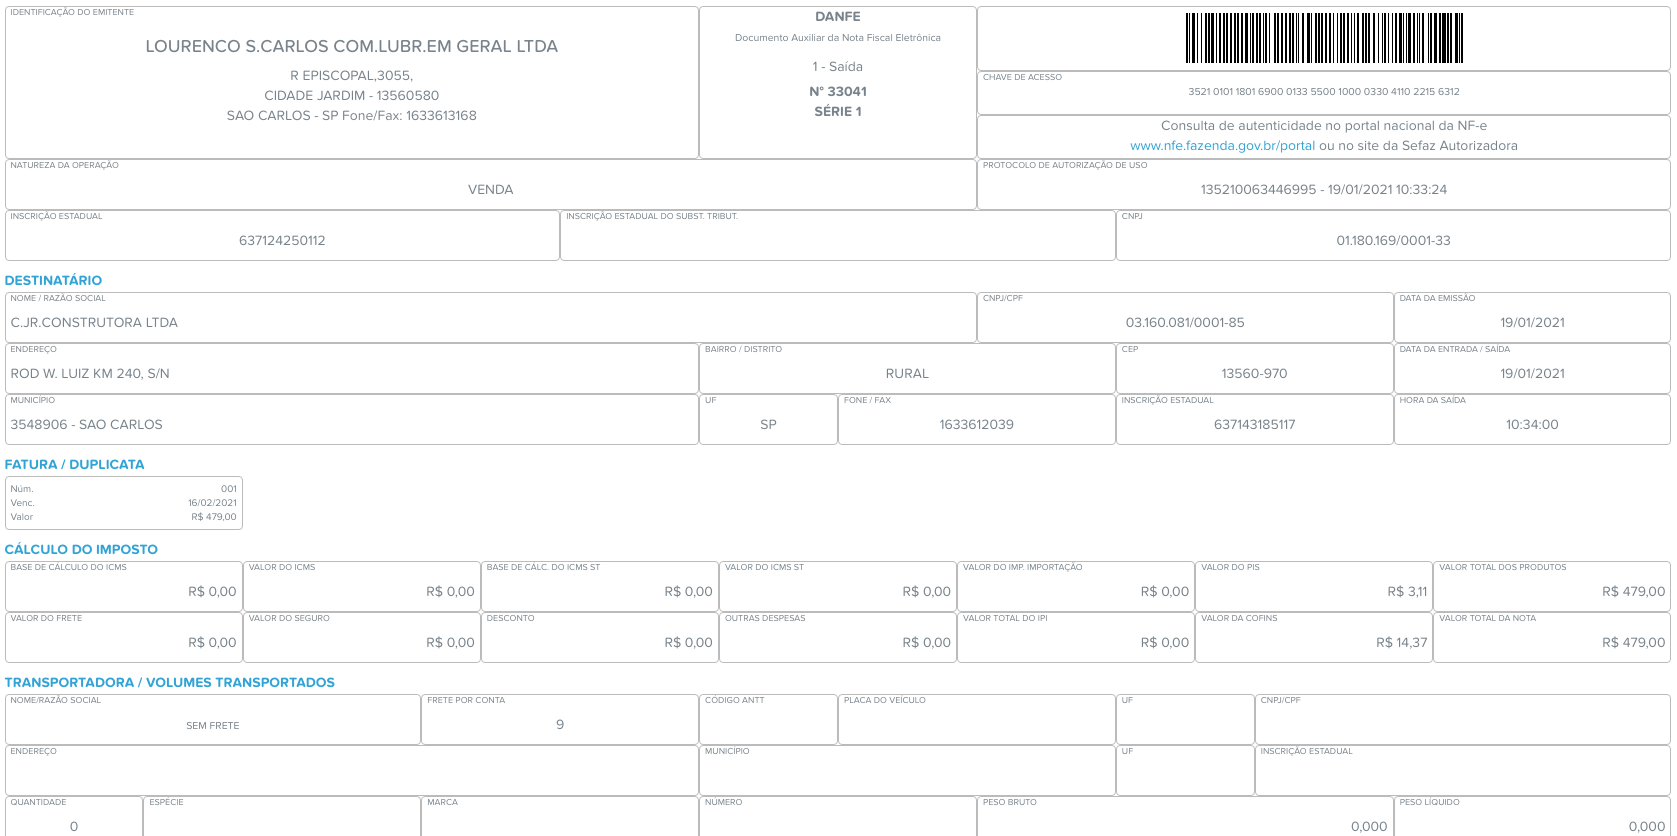
\includegraphics[scale=0.25]{images/nfe.png}
    \fautor
\end{figure}

A disponibilização dos documentos é feita conforme um critério determinado pela Sefaz em que a empresa tem acesso ao documento de acordo com o papel que ela exerce nele. Por exemplo, NFes são disponibilizadas ao destinatário de uma NFe mas não ao emitente. Desta forma, para obter a completude de todos os documentos fiscais de uma empresa de forma automatizada, é necessário que o sistema emitente também armazene os dados.

\section{A Arquivei}
\label{section:documentos-fiscais:arquivei}

Os dados obtidos neste trabalho foram adquiridos através da empresa parceira, Arquivei \cite{portal-arquivei}. A Arquivei é uma empresa especializada em inteligência em documentos fiscais, fundada em 2013 na cidade São Carlos no interior de São Paulo. A empresa disponibiliza um sistema automatizado de consulta de documentos fiscais, utilizando os certificados digitais de seus clientes para obter e armazenar os dados de documentos fiscais. Através do portal, os clientes podem então não apenas cumprir com sua obrigação tributária, mas emitir relatórios e automatizar processos internos das empresas a partir desses dados.

Através dos dados dos clientes da empresa, é possível obter dados de terceiros por meio de um efeito de rede, uma vez que documentos fiscais podem citar diversas empresas. Esse efeito de rede é importante pois aumenta a abrangência dos dados analisados.

A empresa tem hoje mais de 150 funcionários, 12 mil clientes, e atende mais de 85 mil empresas de todo o Brasil. Este trabalho utiliza uma amostra da base de dados da empresa, cuja abrangência será descrita em detalhes no capítulo~\ref{chapter:base-de-dados}.

\subsection{Segurança dos dados}
\label{section:documentos-fiscais:seguranca}

O tratamento dos dados nos ambientes da empresa parceira foram executados apenas pelo autor deste trabalho, de maneira anonimizada, mantendo o sigilo e privacidade previstos na legislação atual e os contratos de prestação de serviço entre a empresa parceira e seus clientes, além de cumprir os critérios previstos no contrato de trabalho entre a empresa parceira e autor deste trabalho. Os dados são armazenados pela empresa parceira utilizando avançados critérios e procedimentos de segurança e com acesso restrito, não tendo tais critérios e procedimentos sido comprometidos de forma alguma na execução deste trabalho.
